\subsection{Methodology}

\subsubsection{Performance Metrics}
\subsection{Data Collection}
\label{subsec:datacollection}

We deployed a data collection system to look for empirical temporal information
about lifetime and bandwidth consumption Tor circuits. Our objective is to have
a deeper understanding of typical Tor usage and whether such usage can benefit
from our channel-based payment system. For example, these measurements might
capture some notion about the type and magnitude of potential premium
traffic. We classify the traffic type based on the service connection
port. Besides the classical ports 80 and 443 used for web traffic, we aggregate
data from some other families including the WHOIS protocol~\cite{rfc3912} and
RWHOIS~\cite{rfc2167} from ports 43 and 4321, respectively. The complete list of
families is constructed from the reduced exit
policies~\cite{reducedexitpolicies} which we run on our relays. This measurement
methodology allows us to reason based on application specific traffic.

% We interested to know about the distribution lifetime of Tor circuits for each
% port we allow. We are also interested to picture how many cells those circuits
% handled through their lifetime with some level of granularity.

\subsubsection{Efforts to preserve users privacy}

To ensure ethical experimentation, we first contacted the Tor research safety
board, a group of Tor researchers who aim minimize privacy risks while fostering
a better understanding of the Tor network and its users~\cite{torsafety}. The
feedback we received was subsequently used to refactor our data collection
process.

Data from multiple exit relays was collected, stripped of origin metadata, and
aggregate on a central server. The data collected from each relay is itself an
aggregation which we perform inside the relay's memory. The data collection is
probabilistic, only 30\% of the circuits processed by our relays were considered
to maintain plausible deniablity on the client's behalf. The aggregation is done
inside bins of configurable size for every different traffic family we
consider. Once we collected enough data from a single family, we dump the
information on the disk, clear the data, and resume a new session. The final
information dumped contains an aggregation of 1600 circuits over an unspecified
time frame that is implicitly determined by the rate of user activity. The
following data was considered:

\begin{itemize}
\item \textbf{Time Profile}: The number of cells in each time interval
  (configured to be 5 seconds) since the success of the DNS request. This
  information sums inbound and outbound cells, and is aggregated over circuits
  by addition.
\item \textbf{Total Counts}: The total amount of cells processed by a
  circuit. This information is aggregated by taking the mean of fixed-size
  nearest neighbor bins, such that the precision of the recorded value depends
  on the number of bins.
\item \textbf{Time Stdevs}: The standard deviation accross the time profiles of
  individual circuits. This information is aggregated in a similar method as the
  Total Counts. This statistic shed some information on the temporal
  deviation of user activity, which can loosely be used to infer interactive vs
  noninteractive traffic.
\end{itemize} Crucially, we do not record information linked to any single
particular user flow on disk. The code used for the data collection is available
online, and can be audited~\cite{code-mt-stats}.

\subsubsection{Observations}

Our measurements successfully captured several important informations needed to
design our experimentation phase. For example, one important question would be:
how should we choose the fraction of premium users in our experimentations? From
Figure~\ref{fig:stats_b}, we observe that $\approx 82\%$ of circuits carrying
only web traffic exchanged less than 1000 cells for both directions (i.e.,
toward the web server and toward the user). This metric does not say that $82\%$
of Tor webusers use less than 1000 cells for a web connection, since it is
theoretically possible that only one user is responsible for consuming less than
1000 cells across our measurements. However, it gives a good idea of the
fraction of circuits that may benefit from a payment channel in the Tor network,
since around $50\%$ of them do not carry data and less than $17\%$ of them carry
at least one web page. These numbers do not mean that $\approx 82\%$ of circuits
carry unethical network usage.

It also appears from Figure~\ref{fig:stats_a} that most of the traffic usually
happens within the first few tens of seconds, and that all type of traffic we
collected seems to follow the same rule. From that result, we believe that the
reliability of payment is critical within the first few seconds, especially from
a relay side viewpoint.

% In another area of research, it may be interesting to point out that since %
$\approx 50\%$ of users do not carry data after their DNS request, some %
adversary doing end-to-end correlation may prefer to use active attacks over %
passive correlation to capture more identities.


\begin{figure*} \centering
	\begin{subfigure}[t]{0.32\textwidth} \centering
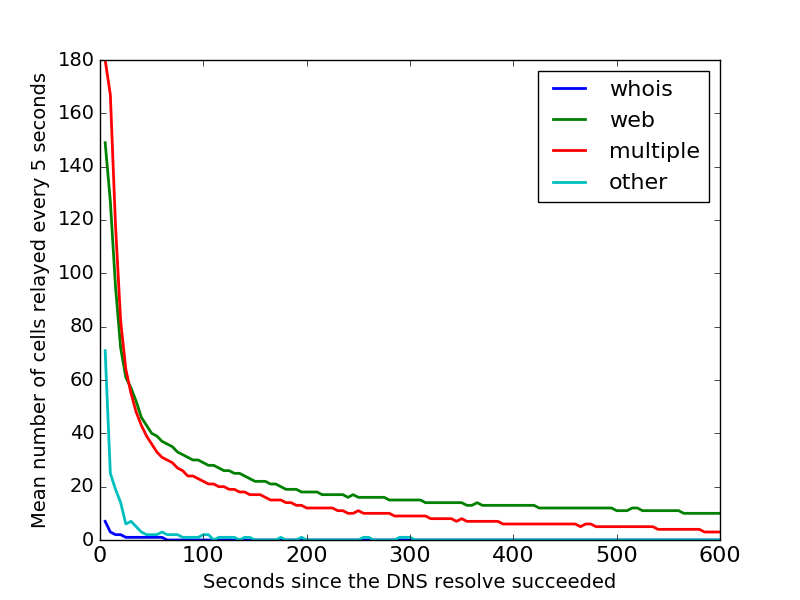
\includegraphics[scale=0.3]{images/exitmeasurement.png}
		\label{fig:stats_a}
		\caption{Time Profile}
	\end{subfigure}
	\begin{subfigure}[t]{0.32\textwidth} \centering
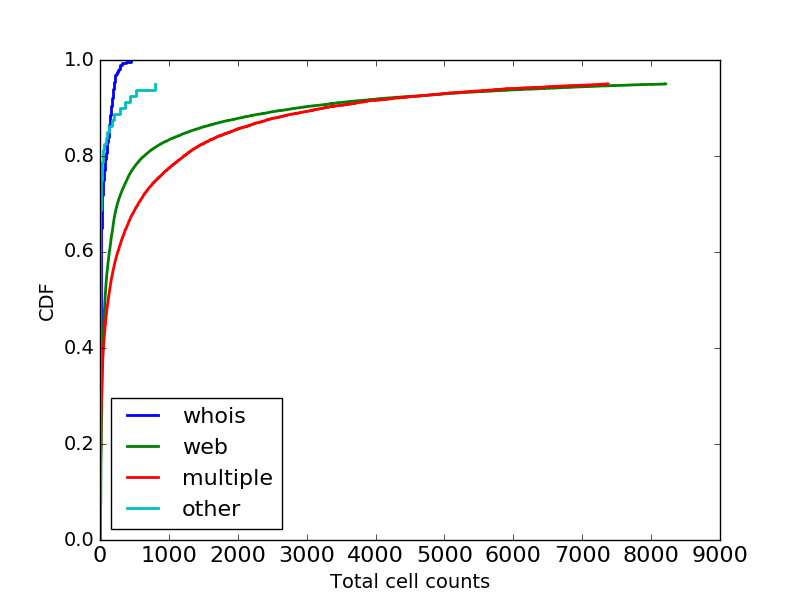
\includegraphics[scale=0.3]{images/totcellcountscdf.png}
		\label{fig:stats_b}
		\caption{Total Counts}
	\end{subfigure}
	\begin{subfigure}[t]{0.32\textwidth} \centering
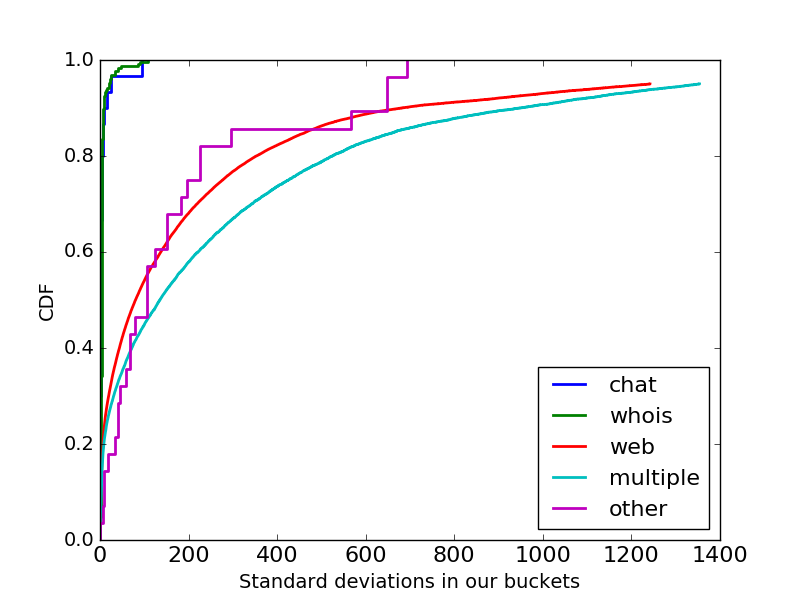
\includegraphics[scale=0.3]{images/stddevs.png}
		\label{fig:stats_c}
		\caption{Time Stdevs}
	\end{subfigure}
	\label{fig:measurements}
	\caption{Tor measurements}
\end{figure*}

\subsection{Experimentations}